\chapter{Gelijkstroomtheorie}
In dit hoofdstuk behandelen we de gelijkstroomtheorie. Nu suggereert het woord
gelijkstroomtheorie dat de theorie alleen de stromen betreft. Dat is echter niet
het geval; het betreft ook de spanningen. We kunnen dus net zo goed spreken over
gelijkspanningstheorie. De keuze voor gelijkstroomtheorie is ingegeven doordat de
grootheid elektrische stroom als een van de zeven grondgrootheden in
het SI-stelsel is gekozen.

In de gelijkstroomtheorie veronderstellen we dat de alle spanningen en stromen
een constante waarden hebben over de tijd. De spanningen en stromen vari\"eren
dus niet als functie van de tijd\footnote{Formeel gezien is een spanning of stroom
die niet van polariteit veranderd ook een gelijkspanning of gelijkstroom. We
veronderstellen hier echter dat de spanningen en stromen constant zijn.}.
 Ze kunnen zowel positief als negatief zijn,
of nul.

In de gelijkstroomtheorie hebben we drie componenten: de ideale
spanningsbron, de ideale stroombron en de ideale weerstand. De
symbolen die gebruikt worden in schakelschema's zijn te zien in
figuur~\ref{fig:symbolenbronnenenweerstand}. Een
ideale spanningsbron levert een constante spanning ongeacht de
stroom die de bron levert. Een ideale stroombron levert een
constante stroom ongeacht de spanning die over de bron staat.
Een ideale weerstand heeft een constante waarde ongeacht de
spanning over en de stroom door de weerstand. Verder merken
we op dat de ideale spanningsbron een interne weerstand heeft
van 0 Ohm. De interne weerstand van de ideale stroombron is
oneindig.

\begin{figure}[!ht]
\centering
\begin{subfigure}{0.30\textwidth}
\centering
\begin{tikzpicture}[line width=1pt]
\draw (0,0) to [V<=$U$] (0,2);
\end{tikzpicture}
\caption{Symbool ideale spanningsbron.}
\label{fig:gelidealespanningsbron}
\end{subfigure}
\begin{subfigure}{0.30\textwidth}
\centering
\begin{tikzpicture}[line width=1pt]
\draw (0,0) to [I, l=$I$, n=I, inner sep=5pt] (0,2);
%\node[left=2pt] at (I.n) {$I$};
\end{tikzpicture}
\caption{Symbool ideale stroombron.}
\end{subfigure}
\begin{subfigure}{0.30\textwidth}
\centering
\begin{tikzpicture}[line width=1pt]
\draw (0,0) to [R, l=$R$] (0,2);
\end{tikzpicture}
\caption{Symbool ideale\\ weerstand.}
\end{subfigure}
%\caption{blabla \protect\subref{fig:gelidealespanningsbron} blabla}
\caption{Symbolen voor de ideale spanningsbron, de ideale stroombron en de ideale weerstand.}
\label{fig:symbolenbronnenenweerstand}
\end{figure}

Voor het aangeven van spanningen gebruiken we de hoofdletter $U$. In Engelstalige boeken
wordt de hoofdletter $V$ gebruikt. Spanning worden uitgedrukt in V (volt). Stromen worden
aangegeven met een hoofdletter $I$ en worden uitgedrukt in A (amp\`ere). Weerstanden
geven we aan met de hoofdletter $R$ (van het Engelse woord \textsl{resistor}) en worden
uitgedrukt in $\Omega$ (ohm).

We kunnen de waarden van spanningen, stromen en weerstanden ook uitdrukken door er een
letter voor te zetten, de zogenoemde SI-voorvoegsels: mV (millivolt), mA (milliamp\`ere),
$\muup$A (microamp\`ere), k$\Omega$ (kilo-ohm), M$\Omega$ (megaohm).

\section{Stroomwet van Kirchhof}
De stroomwet van Kirchhoff zegt dat alle stromen naar een knooppunt toe opgeteld 0 zijn.
Er kan dus geen stroom bijkomen of verloren gaan. In formulevorm:
\begin{equation}
I_1 + I_2 + \cdots + I_n = 0
\end{equation}
Ander gezegd: de totale stroom die naar een knooppunt toevloeit is even groot als de
totale stroom die van het knooppunt wegvloeit. In figuur~\ref{fig:gelstroomwetKirchhoff}
is de stroomwet uitgebeeld.

\begin{figure}[!ht]
\centering
\begin{tikzpicture}[line width=1pt]
\draw (-2,1) to [short, i=$I_1$, -*] (0,0);
\draw (-1.5,-1.5) to [short, i=$I_2$, -*] (0,0);
\draw (2,0.5) to [short, i=$I_3$, -*] (0,0);
\draw (1,-1.5) to [short, i=$I_4$, -*] (0,0);
\end{tikzpicture}
\caption{De stroomwet van Kirchhoff: de stromen naar een knooppunt toe zijn opgeteld 0.}
\label{fig:gelstroomwetKirchhoff}
\end{figure}

In het geval dat een knooppunt slechts twee aansluitingen heeft, is de ingaande stroom even groot als de
uitgaande stroom. Zie figuur~\ref{fig:gelingaandeIisuitgaandeI}.

\begin{figure}[!ht]
\centering
\begin{tikzpicture}[line width=1pt]
\draw (0,0) to [short, i>=$I_1$, -*] ++(3,0) node[above,yshift=.6cm] {$I_1=I_2$} to [short, i>=$I_2$] ++(3,0);
\end{tikzpicture}
\caption{De ingaande stroom is even groot als de uitgaande stroom.}
\label{fig:gelingaandeIisuitgaandeI}
\end{figure}



\section{De spanningswet van Kirchhof}
De spanningswet van Kirchhoff zegt dat alle spanningen in een gesloten kring opgeteld~0
zijn. Er kan dus geen spanning bijkomen of verloren gaan. In formulevorm:
\begin{equation}
U_1 + U_2 + \cdots + U_n = 0
\end{equation}

Anders gezegd: de totale spanning rechtsom opgeteld, is even groot als de totale spanning linksom opgeteld. In figuur~\ref{fig:spanningswetKirchhoff} is de spanningswet uitgebeeld.

\begin{figure}[!ht]
\centering
\begin{tikzpicture}[line width=1pt]
\draw (0.0,0.0)  node[left] {$+$} to [short, o-] ++(0.0,1.0) to [short, -o]  node[above] {$-$} ++(1.0,0.0)
      to [open,l=$U_2$,above] ++(0.5,0.0) node[above] {$+$} to [short, o-] ++(1.0,0.0) to [short, -o] node[right] {$-$} ++(0.0,-1.0)
      to [open,l=$U_3$,inner sep=8pt] ++(0.0,-0.5) node[right] {$+$} to [short, o-] ++(0.0,-1.0) to [short, -o] node[below] {$-$} ++(-1.0,0.0)
      to [open,l=$U_4$,above] ++(-0.5,0.0) node[below] {$+$} to [short, o-] ++(-1.0,0.0) to [short, -o] node[left] {$-$} ++(0.0,1.0)
      to [open,l=$U_1$,inner sep=8pt] ++(0.0,0.5);
\end{tikzpicture}
\caption{De spanningswet van Kirchhoff: alle spanningen in een kring zijn opgeteld 0.}
\label{fig:spanningswetKirchhoff}
\end{figure}

Als een verbinding zich vertakt over twee parallel geschakelde netwerkelementen is de spanning over
de netwerkelementen gelijk. Dit is te zien in figuur~\ref{fig:gelspanningengelijk}.

\begin{figure}[!ht]
\centering
\begin{tikzpicture}[line width=1pt]
\draw (0,0) to[short,-*]++(1,0) to[short] ++(0,0.5) to[short,-o,] node[above] {$+$} ++(1,0) to[open, l=$U_1$,above] ++(1,0) node[above] {$-$} to[short, o-] ++(1,0) to[short,-*] ++(0,-.5) to[short] ++(1,0) to[open] ++(-1,0) to[short] ++(0,-0.5) to[short,-o] node[below] {$-$} ++(-1,0) to [open,l=$U_2$,-o] ++(-1,0) node[below] {$+$} to [short] ++(-1,0) to [short] ++(0,0.5);
\draw (0,1) node {$U_1=U_2$};
\end{tikzpicture}
\caption{De spanningen over twee parallel geschakelde elementen zijn gelijk.}
\label{fig:gelspanningengelijk}
\end{figure}




\section{De wet van Ohm}
De verhouding tussen de spanning over een weerstand en de stroom door de weerstand is constant
en wordt de wet van Ohm genoemd. De wet wordt meestal geschreven als:
\begin{equation}
U=I\cdot R
\end{equation}
%
Gegeven een bepaalde spanning en stroom, dan kan de weerstandswaarde berekend worden met:
%
\begin{equation}
R = \dfrac{U}{I}
\end{equation}
%
In figuur~\ref{fig:geldewetvanohm} is de wet van Ohm uitgebeeld. Aan de spanningbron $U$ wordt
een weerstand $R$ geplaatst. We spreken dan dat de spanningsbron wordt belast. Ook hier geldt de
spanningswet van Kirchhoff: de spanning $U$ van de bron is gelijk aan de spanning $U_R$ over de
weerstand. Bij de gegeven richting van de stroom $I$ geldt dat het potentiaal bij de `$+$' groter
is dan het potentiaal bij de `$-$'.

\begin{figure}[!ht]
\centering
\begin{tikzpicture}[bookcircuit]
\draw (0,0) to [V<=$U$] ++(0,2) to [short, i=$I$] ++(2.5,0) to [R=$R$, v=$U_R$] ++(0,-2) to [short,-.] (0,0)
;
%%%\draw (-2,0) to[short, i=$I$] (0,0);
%%%\draw (0,0) to[R=$R$, v_>=$U$] (2,0);
\end{tikzpicture}
\caption{De spanning over en stroom door een weerstand is constant.}
\label{fig:geldewetvanohm}
\end{figure}

\section{Serieschakeling van weerstanden}
In figuur~\ref{fig:gelserieschakelingweerstanden} is een schakeling te zien waarbij de weerstanden
in serie geschakeld zijn en gevoed worden door een spanningsbron. De spanningsbron levert een stroom
$I$ waardoor de spanningsbron een bepaalde weerstand ondervindt. We noemen deze weerstand $R_s$.

\begin{figure}[!ht]
\centering
\begin{tikzpicture}[bookcircuit]
\draw (0,0) to [V<=$U$] ++ (0,2) to [short, i=$I$] ++(2,0)
            to [R, l=$R_1$,v=$U_1$] ++(2,0) to [R, l=$R_2$, v=$U_2$] ++(2,0)
            coordinate (A);
\draw[dotted] (A) --  ++(1,0) coordinate (B);
\draw (B) to [R,l=$R_n$,v=$U_n$] ++(2,0) to [short] ++(0.5,0) to [short] ++(0,-2) to [short,-.] (0,0);
\end{tikzpicture}
\caption{Serieschakeling van weerstanden.}
\label{fig:gelserieschakelingweerstanden}
\end{figure}

Vanuit de spanningswet van Kirchhoff volgt dat:
%
\begin{equation}
U=U_1+U_2+\cdots+U_n
\end{equation}
%
Vanuit stroomwet van Kirchhoff volgt dat:
%
\begin{equation}
I = I_1 = I_2 = \cdots = I_n
\end{equation}
%
De stroom die de bron levert is dus even groot als de stromen door de weerstanden.
De bron met spanning $U$ levert een stroom $I$ zodanig dat:
%
\begin{equation}
U=I\cdot R_s
\end{equation}
%
Dus volgt dat:
%
\begin{equation}
I\cdot R_s = I\cdot R_1+I\cdot R_2+\cdots+I\cdot R_n
\end{equation}
%
We schappen aan beide kanten $I$ zodat volgt dat:
%
\begin{equation}
R_s = R_1 + R_2 + \cdots R_n
\end{equation}
%
Hierbij is $R_s$ de vervangingswaarde van de in serie geschakelde weerstanden.


\section{Parallelschakeling van weerstanden}
In figuur~\ref{fig:gelparalledschakelingweerstanden} is een parallelschakeling van een
aantal weerstanden te zien. De schakeling wordt gevoed door de spanningsbron $U$. Als
gevolg van de weerstanden zal de bron een bepaalde stroom leveren. Hierdoor ondervindt
de spanningsbron een bepaalde weerstand. Deze weerstand noemen we $R_p$.

\begin{figure}[!ht]
\centering
\begin{tikzpicture}[bookcircuit]
%% Draw voltage source, wire with current I, resistor R1 and back to minus of voltage source
\draw (0,0) to [V<=$U$] ++ (0,2) to [short] ++(0,0.25) to [short,i=$I$,-*] ++(3,0) coordinate (A) to [short] ++(0,-0.25) to[R=$R_1$,-*,i>^=\small $I_1$,v=\small $U_1$] ++(0,-2) to [short,-.] (0,0);
%% Draw resistor R2 and wire to minus of resistor R1
\draw (A) to[short,-*] ++(2,0) coordinate (B) to [short] ++(0,-0.25) to [R=$R_2$,-*,i>^=\small $I_2$, v=\small $U_2$] ++(0,-2) to [short] ++(-2,0);
%% Draw short heading to Rk
\draw (B) to[short] ++(0.75,0) coordinate (C);
%% Draw dotted wire
\draw[dotted] (C) -- ++(1,0) coordinate (D);  
%% Draw Rk
\draw (D) to [short] ++(0.75,0) to [short] ++(0,-0.25) to [R=$R_n$,i>^=\small $I_n$, v=\small $U_n$ ] ++(0,-2) to [short] ++(-0.75,0) coordinate (E);
%% Draw dotted wire
\draw[dotted] (E) -- ++(-1,0) coordinate (F);
%% Draw wire to minus of R2
\draw (F) to [short] ++(-0.75,0);
\end{tikzpicture}
\caption{Parallelschakeling van weerstanden.}
\label{fig:gelparalledschakelingweerstanden}
\end{figure}

Vanuit de spanningswet van Kirchhoff vinden we dat:
%
\begin{equation}
U = U_1 = U_2 = \cdots = U_n
\end{equation}
%
De spanningen over de weerstanden zijn even groot als de bronspanning.
Vanuit de stroomwet van Kirchhoff vinden we dat:
%
\begin{equation}
I = I_1 + I_2 + \cdots + I_n
\end{equation}
%
We kunnen de stroomwet ook formuleren als:
%
\begin{equation}
\dfrac{U}{R_p} = \dfrac{U}{R_1} + \dfrac{U}{R_2} + \cdots + \dfrac{U}{R_n}
\end{equation}
%
We schrappen aan beide zijden van de vergelijking de spanning $U$ zodat we krijgen dat:
%
%De vervangingswaarde voor de parallelschakeling van een aantal weerstanden is te berekenen met:
\begin{equation}
\dfrac{1}{R_p} = \dfrac{1}{R_1} + \dfrac{1}{R_2} + \cdots + \dfrac{1}{R_n}
\end{equation}
%
Hierin is $R_p$ de vervangingswaarde van de parallel geschakelde weerstanden.
Voor twee parallel geschakelde weerstanden geldt dat:
\begin{equation}
\dfrac{1}{R_p} = \dfrac{1}{R_1} + \dfrac{1}{R_2}
\end{equation}
%
Dit kan worden omgewerkt tot:
\begin{equation}
R_p = \dfrac{R_1\cdot R_2}{R_1+R_2}
\end{equation}


\section{Spanningsdeling}
In figuur~\ref{fig:gelspanningsdeling} is een schema te zien van een bron met twee in
serie geschakelde weerstanden. De spanning $U$ zal zich in een bepaalde verhouding
verdelen over de twee weerstanden. Er is sprake van spanningsdeling.

\begin{figure}[!ht]
\centering
\begin{tikzpicture}[bookcircuit]
\draw (0,0) to [V<=$U$] ++ (0,2) to [short, i=$I$] ++(1.5,0)
            to [R, l=$R_1$,v=$U_1$] ++(2,0) to [R, l=$R_2$, v=$U_2$] ++(2,0)
            to [short] ++(0.5,0) to [short] ++(0,-2) to [short,-.] (0,0);
\end{tikzpicture}
\caption{Schema voor spanningsdeling.}
\label{fig:gelspanningsdeling}
\end{figure}

De stroom $I$ kunnen we berekenen met:
%
\begin{equation}
I = \dfrac{U}{R_!+R_2}
\end{equation} 
%
Voor de spanningen $U_1$ en $U_2$ kunnen we schrijven dat:
%
\begin{equation}
U_1 = I\cdot R_1 = \dfrac{R_1}{R_1+R_2}\cdot U \qquad\text{en}\qquad U_2 = I\cdot R_2 = \dfrac{R_2}{R_1+R_2}\cdot U
\end{equation}


\section{Stroomdeling}
In figuur~\ref{fig:gelstroomdeling} is een schema te zien van een bron met twee parallel
geschakelde weerstanden. De stroom $I$ zal zich in een bepaalde verhouding
verdelen over de twee weerstanden. Er is sprake van stroomdeling.

\begin{figure}[!ht]
\centering
\begin{tikzpicture}[bookcircuit]
%% Draw voltage source, wire with current I, resistor R1 and back to minus of voltage source
\draw (0,0) to [V<=$U$] ++ (0,2) to [short] ++(0,0.25) to [short,i=$I$,-*] ++(3,0) coordinate (A) to [short] ++(0,-0.25) to[R=$R_1$,-*,i>^=\small $I_1$,v=\small $U_1$] ++(0,-2) to [short,-.] (0,0);
%% Draw resistor R2 and wire to minus of resistor R1
\draw (A) to[short] ++(2,0) coordinate (B) to [short] ++(0,-0.25) to [R=$R_2$,i>^=\small $I_2$, v=\small $U_2$] ++(0,-2) to [short] ++(-2,0);
\end{tikzpicture}
\caption{Schema voor stroomdeling.}
\label{fig:gelstroomdeling}
\end{figure}

De spanning $U$ kunnen kunnen we berekenen met:
%
\begin{equation}
U = I\cdot\dfrac{R_1\cdot R_2}{R_1+R_2}
\end{equation}
%
Natuurlijk geldt de stroomwet van Kirchhoff:
%
\begin{equation}
I = I_1 + I_2 = \dfrac{U}{R_1} + \dfrac{U}{R_2}
\end{equation}
%
Voor $I_1$ geldt dan:
%
\begin{equation}
I_1 = \dfrac{U}{R_1} = \dfrac{R_1\cdot R_2}{R_1+R_2}\cdot \dfrac{1}{R_1}\cdot I = \dfrac{R_2}{R_!+R_2}\cdot I
\end{equation}
%
Op vergelijkbare wijze vinden we voor $I_2$:
%
\begin{equation}
I_2 = \dfrac{U}{R_2} = \dfrac{R_1\cdot R_2}{R_1+R_2}\cdot \dfrac{1}{R_2}\cdot I = \dfrac{R_1}{R_!+R_2}\cdot I
\end{equation}


\section{De niet-ideale spanningsbron}
In de praktijk hebben we te maken met niet-ideale spanningsbronnen. We kunnen zo'n bron
weergeven met een ideale spanningsbron in serie met een ideale weerstand. De ideale
weerstand wordt de \textsl{inwendige weerstand} genoemd. Dit is te zien in
\index{inwendige weerstand}
figuur~\ref{fig:gelnisopenkort}.

\begin{figure}[!ht]
\begin{subfigure}{0.5\textwidth}
\centering
\begin{tikzpicture}[bookcircuit]
\draw (0,0) to [V<=$U$] ++(0,2) to [R=$R_i$,-*] coordinate (A) ++(2.5,0) node[right] {$+$} to [open] ++(0,-2) coordinate (B) node[right] {$-$} to [short,*-.] (0,0);
\draw ($(A)!0.5!(B)$) node[right] {$U_o$};
\end{tikzpicture}
\caption{}
\label{fig:gelnisopen}
\end{subfigure}%
\begin{subfigure}{0.5\textwidth}
\centering
\begin{tikzpicture}[bookcircuit]
\draw (0,0) to [V<=$U$] ++(0,2) to [R=$R_i$,-*] ++(2.5,0) to [short, i=$I_k$] ++(0,-2) to [short,*-.] (0,0);
\end{tikzpicture}
\caption{}
\label{fig:gelniskort}
\end{subfigure}
\caption{Niet-ideale spanningsbron: \subref{fig:gelnisopen} onbelast, \subref{fig:gelniskort} kortgesloten.}
\label{fig:gelnisopenkort}
\end{figure}

In figuur~\ref{fig:gelnisopen} is te zien dat de niet-ideale spanningsbron onbelast is.
De spanning $U_o$ is even groot als de bronspanning $U$. Er loopt immers geen stroom zodat
er geen spanningsval over de inwendige weerstand staat. Deze spanning wordt de \textsl{open
klemspanning} genoemd. In figuur~\ref{fig:gelniskort} is
\index{open klemspanning}
de niet-ideale spanningsbron kortgesloten. Over de inwendige weerstand staat nu de volledige
bronspanning. Er loopt dan een zekere \textsl{kortsluitstroom} $I_k$. We kunnen de inwendige
\index{kortsluitstroom}
weerstand berekenen door de uitgangsspanning $U_o$ te delen door de kortsluitstroom $I_k$.

Voor een goede spanningsbron moet de inwendige weerstand klein zijn. Praktische waarden van
de inwendige weerstanden liggen tussen de enkele tientallen m$\Omega$ tot enkele~$\Omega$.
Zo kan een autoaccu met een spanning van 12 V stromen van meer dan 100 A leveren. Het is dan
ook niet aan te bevelen om dergelijke kortsluitstromen te meten. De inwendige weerstand
van eenvoudige batterijen ligt in de orde van enkele $\Omega$. Een laboratoriumvoeding moet
natuurlijk ook een lage inwendige weerstand hebben om de uitgangsspanning zo constant
mogelijk te houden. Veelal is de voeding beschermd tegen kortsluiting en wordt de
kortsluitstroom begrensd.


\section{De niet-ideale stroombron}
In de praktijk hebben we ook te maken met niet-ideale stroombronnen. De niet-ideale
stroombron is te modelleren als een ideale stroombron parallel geschakeld aan een ideale
weerstand. Ook deze weerstand wordt de inwendige weerstand genoemd. Dit is te zien in
figuur~\ref{fig:gelnissopenkort}.

\begin{figure}[!ht]
\begin{subfigure}{0.5\textwidth}
\centering
\begin{tikzpicture}[bookcircuit]
\draw (0,0) to [I, l=$I$, inner sep=5pt] ++(0,2) to [short] ++(1,0) coordinate (A) to [R=$R_i$,*-*]  ++(0,-2) coordinate (B) to [short,-.] (0,0) (A) to [short, -*] ++(1,0) node[right] {$+$} (B) to [short, -*] ++(1,0) node[right] {$-$}; 
\draw ($(A)!0.5!(B)$) node[right,xshift=1cm] {$U_o$};
\end{tikzpicture}
\caption{}
\label{fig:gelnissopen}
\end{subfigure}%
\begin{subfigure}{0.5\textwidth}
\centering
\begin{tikzpicture}[bookcircuit]
\draw (0,0) to [I, l=$I$, inner sep=5pt] ++(0,2) to [short] ++(1,0) coordinate (A) to [R=$R_i$,*-*]  ++(0,-2) coordinate (B) to [short,-.] (0,0) (A) to [short, -*] ++(1,0) to [short, i=$I_k$, -*] ++(0,-2) to [short] (B) ; 
\end{tikzpicture}
\caption{}
\label{fig:gelnisskort}
\end{subfigure}
\caption{Niet-ideale stroombron: \subref{fig:gelnissopen} onbelast, \subref{fig:gelnisskort} kortgesloten.}
\label{fig:gelnissopenkort}
\end{figure}

In figuur~\ref{fig:gelnissopen} is de niet-ideale stroombron onbelast. De stroom $I$
loopt nu door de inwendige weerstand. Hierdoor zal over de bron een bepaalde spanning aanwezig
zijn. We noemen die spanning de open klemspanning. In figuur~\ref{fig:gelnisskort} is de bron
kortgesloten. De stroom $I$ loopt nu volledig door de kortsluiting. We noemen de stroom de
kortsluitstroom. We kunnen de inwendige
weerstand berekenen door de uitgangsspanning $U_o$ te delen door de kortsluitstroom $I_k$.

Voor een goede stroombron moet de inwendige weerstand zo groot mogelijk zijn. Praktische
waarden voor $R_i$ liggen tussen enkele honderden k$\Omega$ tot vele M$\Omega$. Aan
figuur~\ref{fig:gelnissopen} kunnen we nog iets ontdekken. De uitgangsspanning in onbelaste
toestand zal zeer groot zijn. We kunnen nu inzien dat een stroombron dus nooit onbelast gelaten
mag worden. Een laboratoriumvoeding zal de uitgangsspanning in onbelaste toestand begrenzen.

\section{Vermogen ontwikkeld in een weerstand}
Een weerstand waar een spanning over staat en een stroom door loopt dissipeert energie. Dit is weergegeven in
figuur~\ref{fig:gelvermogensdissipatie}. Dat een weerstand energie dissipeert kunnen we merken doordat de
weerstand warm wordt.
Het \textsl{vermogen} dat ontwikkeld wordt in een weerstand is het product van de spanning over
\index{vermogen}
en de stroom door de weerstand:
%
\begin{equation}
P = U\cdot I 
\end{equation}

\begin{figure}[!ht]
\centering
\begin{tikzpicture}[bookcircuit]
\draw (0,0) to [V<=$U$] ++(0,2) to [short, i=$I$] ++(2.5,0) to [R,l_=$R$,n=R] ++(0,-2) to [short,-.] (0,0);
\draw[decorate, decoration={snake, segment length=5pt, amplitude=1pt},->stealth'] (R) ++(0.2,0.2) -> ++(2,0.2);
 \draw[decorate, decoration={snake, segment length=5pt, amplitude=1pt},->stealth'] (R) ++(0.2,0.0) -> ++(2,0.0) node[right] {W};
\draw[decorate, decoration={snake, segment length=5pt, amplitude=1pt},->stealth'] (R) ++(0.2,-0.2) -> ++(2,-0.2); \end{tikzpicture}
\caption{De weerstand dissipeert warmte.}
\label{fig:gelvermogensdissipatie}
\end{figure}


Vermogen wordt uitgedrukt in W (watt). Aangezien we voor $U$ ook kunnen schrijven $U=I\cdot R$
kunnen we ook stellen dat:
\begin{equation}
P = I^2\cdot R
\end{equation}
Verder kunnen we voor $I$ schrijven dat $I=\dfrac{U}{R}$ zodat we kunnen stellen dat:
\begin{equation}
P = \dfrac{U^2}{R}
\end{equation}
%
De eenheid W (watt) kan ook geschreven worden als J/s (joules per seconde) en dat geeft precies
aan wat het vermogen inhoudt: energieafgifte per seconde. Willen we de totale energieafgifte
over een bepaalde tijd $t$ berekenen dan moeten we het vermogen vermenigvuldigen met de tijd:
%
\begin{equation}
W = P\cdot t
\end{equation}
%
De variabele $W$ staat voor het Engelse woord \textsl{Work}. Een veel gebruikte eenheid van energie
is de kWh (kilowattuur). Dit komt overeen met de energie
als een component een vermogen van 1000 W een uur lang dissipeert. De hoeveelheid energie is:
%
\begin{equation}
1\ \mathrm{kWh} = 1000\ \mathrm{W} \times 1\ \mathrm{uur} = 1000\ \dfrac{\mathrm{J}}{\mathrm{s}} \times 3600\ \mathrm{s} = 3.600.000\ \mathrm{J} = 3,6\ \mathrm{MJ}
\end{equation}

%%%De spanning over een spoel kan berekend worden met:
%%%\begin{equation}
%%%U = L\dfrac{\text{d}i}{\text{d}t}
%%%\end{equation}
%%%Hierin is $L$ de zelfinductie van de spoel. Bij een sinusvormige spanning met hoekfrequentie
%%%$\omega$ kunnen we dus schrijven:
%%%\begin{equation}
%%%U = L\dfrac{\text{d}\, i \sin \omega t}{\text{d}t} = \omega L i\cos \omega t
%%%\end{equation}
%%%De amplitude van de spanning is dus afhankelijk van de hoekfrequentie $\omega$.
%%%
%%%De spanning over een condensator kan berekend worden met:
%%%\begin{equation}
%%%U = \dfrac{1}{C}\int i\,\text{d}t 
%%%\end{equation}
%%%
%%%Hierin is $C$ de capaciteit van de condensator. Bij een sinusvormige spanning met hoekfrequentie
%%%$\omega$ kunnen we schrijven:
%%%\begin{equation}
%%%U = \dfrac{1}{C}\int i\sin \omega t\,\text{d}t = -\dfrac{i}{\omega C} \cos \omega t
%%%\end{equation}


\section{Maximale vermogensoverdracht}
In figuur~\ref{fig:maximalevermogensoverdracht} is te zien dat een niet-ideale
spanningsbron met spanning $U$ en inwendige weerstand $R_i$ is verbonden met
een uitwendige weerstand $R_u$. We willen graag maximale vermogensoverdracht
vanuit de bron in $R_u$.

\begin{figure}[!ht]
\centering
\begin{circuitikz}[bookcircuit]
\draw (0,0) to[V<=$U$] ++(0,2) to[R=$R_i$, -*] ++(2,0) to[short, i=$I$] ++(1,0) to[R=$R_u$] ++(0,-2) to[short, -*] ++(-1,0) to[short,-.] (0,0);
\end{circuitikz}
\captionsetup{width=.9\linewidth}
\caption{Een niet-ideale spanningsbron met inwendige weerstand wordt belast met een uitwendige weerstand.}
\label{fig:maximalevermogensoverdracht}
\end{figure}

De stroom die de bron produceert is:
%
\begin{equation}
I = \dfrac{U}{R_i + R_u}
\end{equation}
%
Het vermogen dat in de uitwendige weerstand wordt gedissipeerd is:
%
\begin{equation}
\label{equ:dissipatedru}
P_{Ru} = I^2R_u = \left(\dfrac{U}{R_i+R_u}\right)^2 R_u
       = \dfrac{R_u}{(R_i+R_u)^2}\: U^2
\end{equation}
%
We kunnen inzien dat als $R_u$ klein is de stroom groot zal zijn maar het vermogen in $R_u$ is
dan klein. Als $R_u$ groot is dan zal de stroom klein zijn en ook dan is het
vermogen in $R_u$ klein. Ergens daartussen ligt een optimum waarbij het meeste vermogen
wordt overgedragen in de uitwendige weerstand. Hiertoe differenti\"eren we de vergelijking
\eqref{equ:dissipatedru} naar $R_u$:
%
\begin{equation}
\setlength{\jot}{10pt}
\begin{split}
\dfrac{\text{d}P_{Ru}}{\text{d}R_u} &= U^2\dfrac{(R_i+R_u)^2-R_u\cdot2(R_i+R_u)}{(R_i+R_u)^4} \\
      &= U^2 \dfrac{(R_i+R_u)-2R_u}{(R_i+R_u)^3•} \\
      &= U^2 \dfrac{R_i-R_u}{(R_i+R_u)^3}
\end{split}
\end{equation}
%
Vervolgens stellen de differentiaalquoti\"ent gelijk aan 0 om de extremen te vinden:
%
\begin{equation}
\dfrac{\text{d}P_{Ru}}{\text{d}R_u} = 0 \qquad \Longleftrightarrow \qquad U^2 \dfrac{R_i-R_u}{(R_i+R_u)^3} = 0
\end{equation}
%
Hieruit volgt dat de maximale vermogensoverdracht plaatsvindt als de uitwendige
weerstand gelijk is aan de inwendige weerstand dus bij $R_u=R_i$. De maximale
vermogensoverdracht is eenvoudig uit te rekenen door de uitwendige weerstand
gelijk te stellen aan de inwendige weerstand. Daaruit volgt dat:
%
\begin{equation}
P_{Ru,max} = \dfrac{U^2}{4R_i}
\end{equation}
%
Over de effici\"entie van de vermogensoverdracht kunnen we ook wat vertellen. De effi\"entie is
het getransporteerde vermogen gedeeld door het opgewekte vermogen:
%
\begin{equation}
\eta = \dfrac{P_{Ru}}{P_{bron}} = \dfrac{I^2\cdot R_u}{I^2\cdot(R_i+R_u)} = \dfrac{R_u}{R_i+R_u}
\end{equation}
%
Bij maximale vermogensoverdracht ($R_i=R_u$) is de effi\"entie dan 50\%. De helft van het beschikbare
vermogen wordt in de uitwendige weerstand gedissipeerd. Dat betekent dat de bron zelf evenveel vermogen
dissipeert.

In figuur~\ref{fig:gelbeschikbarevermogenseneff} zijn de diverse vermogens en effici\"entie van de
vermogensoverdracht uitgebeeld. De vermogens zijn genormaliseerd op 1. Dat houdt in dat bij
kortsluiting van de bron het beschikbare vermogen dat in de inwendige weerstand wordt gedissipeerd
gelijk wordt gesteld aan 1. De vermogens zijn uitgezet tegen de verhouding van de uitwendige weerstand
en de inwendige weerstand. Een verhouding van $R_u/R_i=1$ betekent dat $R_u=R_i$.

\begin{figure}[!ht]
\centering
\begin{tikzpicture}
	%\sansmath
	\begin{axis}[width=10cm,height=7cm,
		xlabel=$R_U/R_I$,
		ylabel=$P_{norm}$,
		legend entries={$\eta$,$P_{Ri}$,$P_{bron}$, $P_{Ru}$},
		legend style={font=\small,at={(0.95,0.75)},anchor=north east},
		xtick={0,1,...,10},
		reverse legend,
        y tick label style={
        /pgf/number format/.cd,
            fixed,
            fixed zerofill,
            precision=1,
	        use comma,
    	    1000 sep={},
            /tikz/.cd
        }
		%legend pos=outer north east
	]
	% invoke external gnuplot as
	% calculator:
	%\addplot [domain=0:2*pi, mark=*, blue,samples=100] gnuplot[id=sin]{sin(x)};
	\addplot [domain=0:10,samples=101,olive,loosely dashdotted,thick] gnuplot[id=eff] {x/(1+x)};
	\addplot [domain=0:10,samples=101,red,dashed,thick] gnuplot[id=pri] {1/((1+x)^2)};
	\addplot [domain=0:10,samples=101,black,dotted,thick] gnuplot[id=pb] {1/(1+x)};
	\addplot [domain=0:10,samples=101,blue,thick] gnuplot[id=pru] {x/((1+x)^2)};
	\end{axis}

    \begin{axis}[width=10cm,height=7cm,
    %ymin=0.0, ymax=1.0,
    hide x axis,
    axis y line*=right,
    ytick={0.0,0.1,...,1.0},
    ylabel={$\eta$},
    ylabel near ticks,
    ylabel style={rotate=-180},
    y tick label style={
    /pgf/number format/.cd,
            fixed,
            fixed zerofill,
            precision=1,
	        use comma,
    	    1000 sep={},
            /tikz/.cd
        }
    ]
    \end{axis}          	

\end{tikzpicture}
\caption{Genormaliseerde ontwikkelde vermogens in de inwendige en uitwendige weerstand en de bron. Links is de effici\"entie van de vermogensoverdracht weergegeven.}
\label{fig:gelbeschikbarevermogenseneff}
\end{figure}

De ononderbroken kromme geeft de vermogensopname van de uitwendige weerstand weer. De gestreepte
kromme geeft de vermogensopname van de inwendige weerstand weer. Het geleverde vermogen van de
bron wordt door de gestippelde kromme weergegeven. Verder is te zien dat de gestippelde
streepjes lijn de effici\"entie weergeeft.

We bespreken een drietal markante punten.
Bij kortsluiting van de bron ($R_u/R_i=0$) wordt het maximale vermogen van de bron in de inwendige
weerstand gedissipeerd. Te zien is dat $P_{bron} = P_{Ri} = 1$ en $P_{Ru} = 0$. De effici\"entie is 0.
Bij $R_u=R_i$ is het gedissipeerde vermogen in de inwendige en uitwendige weerstand $0,25$. Het geleverde
bronvermogen is $0,5$ en de effici\"entie is $0,5$. Naar mate $R_u$ groter wordt, neemt het geleverde
en opgenomen vermogen af. Bijna al het vermogen wordt in $R_u$ gedissipeerd. De effci\"entie neemt toe
maar zal nooit 1 worden.


\section{De belastingskarakteristiek}

In deze paragraaf bespreken we het begrip \textsl{belastingskarakteristiek}. We kunnen hiermee de stromen
en spanningen in een netwerk bepalen via een grafische weg. Dit is met name bij het gebruik van niet-lineaire
netwerkelementen zoals de diode erg handig.

In figuur~\ref{fig:gelschemavoorbelastingskarakteristiek} is een schakeling te zien met een spanningsbron
$U$ en een inwendige weerstand $R_i$. De bron wordt belast door de belastingsweerstand $R_b$. Deze weerstand
is variabel gemaakt en kan vari\"eren tussen $R_b = 0$ en $R_b \rightarrow \infty$.

\begin{figure}[!ht]
\centering
\begin{tikzpicture}[bookcircuit]
\draw (0,0) to[V<=$U$] ++(0,2) to[R=$R_i$, -*] ++(2,0) coordinate (A) node[below] {$+$} to[short, i=$I$] ++(2,0) to[vR=$R_b$,invert,mirror] ++(0,-2) to[short, -*] ++(-2,0) coordinate (B) node[above] {$-$} to[short,-.] (0,0);
\draw[draw=none] (A) -- (B) node[midway] {$U_{R_b}$};
\end{tikzpicture}
\captionsetup{width=.9\linewidth}
\caption{Schema voor de belastingskarakteristiek.}
\label{fig:gelschemavoorbelastingskarakteristiek}
\end{figure}

Voor de spanningen in het schema kunnen we opstellen dat:
%
\begin{equation}
U = U_{R_i} + U_{R_b}
\end{equation}
%
Deze functie kunnen we ook schrijven als:
\begin{equation}
U_{R_i} = - U_{R_b} + U
\end{equation}
%
Vervolgens delen we alle spanningen door $R_i$:
%
\begin{equation}
\dfrac{U_{R_i}}{R_i} = - \dfrac{U_{R_b}}{R_i} + \dfrac{U}{R_i}
\end{equation}
%
Nu is de term $U_{R_i}/R_i$ gelijk aan de bronstroom $I$. De term $U/R_i$ is de stroom die de bron levert
als de bron kortgesloten wordt, d.w.z.\@ $R_b=0$. Dit wordt de kortsluitstroom $I_k$ genoemd. We kunnen de
functie dus schrijven als:
%
\begin{equation}
I = -\dfrac{1}{R_i}\cdot U_{R_b} + I_k
\end{equation}
%
We hebben nu een rechte lijn gekregen met de algemene gedaante:
%
\begin{equation}
y=ax+b
\end{equation}
De stroom $I$ komt overeen met de afhankelijke variabele $y$. De spanning $U_{R_b}$ komt overeen met de
onafhankelijke variabele $x$. De factor $-1/R_i$ komt overeen met de constante $a$ en wordt de
richtingsco\"effici\"ent genoemd. De kortsluitstroom $I_k$ komt overeen met het startgetal $b$.

We kunnen de lijn nu uitzetten in een grafiek, zie figuur~\ref{fig:gelbelastingskarakteristiek}.
We onderscheiden twee markante punten op de lijn:

\begin{itemize}
\item Het kortsluitpunt. Dit doet zich voor als $R_b=0$, dus als de bron is kortgesloten. De bron
      levert dan een maximale stroom, de kortsluitstroom $I_k$ genoemd. De spanning over $R_b$ is
      dan 0 V.
\item Het nullastpunt. Dit doet zich voor als $R_b \rightarrow \infty$, dus als $R_b$ uit de schakeling
      is verwijderd. Dan geldt dat $I=0$ A en $U_{R_b}=U$. Dit wordt de open klemspanning $U_o$ genoemd. 
\end{itemize}

\begin{figure}[!ht]
\centering
\begin{tikzpicture}[line width=1pt,yscale=0.8]
\draw[-latex] (0,0) node[left] {$0$} -- (0,6) node[above] {$I$};
\draw[-latex] (0,0) node[below] {$0$} -- (6,0) node[right] {$U_{R_b}$};
\draw (0,5) node[left] {$I_k$} -- (5,0) coordinate[pos=0.2] (rico) coordinate[midway] (rbisri) node[below] {$U_o$};
\draw[<-] (0.2,5) -- ++(0.8,0.4) node[right] {$R_b=0$};
\draw[<-] (5.05,0.2) -- ++(0.8,0.4) node[right] {$R_b\rightarrow\infty$};
\draw[<-] (rico) ++(0.05,0.2) -- ++(0.8,0.4) node[right] {rico = $-\dfrac{1}{R_i}$};
\draw[dashed] (rbisri) -- (rbisri -| {{0,0}}) node[left] {$\frac{1}{2}I_k$};    %{$\dfrac{I_k}{2}$};
\draw[dashed] (rbisri) -- (rbisri |- {{0,0}}) node[below] {$\frac{1}{2}U_o$};   %{$\dfrac{U_o}{2}$};
\draw[<-] (rbisri) ++(0.1,0.1) -- ++(0.8,0.4) node[right] {$R_b=R_i$};
\end{tikzpicture}
\caption{Belastingskarakteristiek.}
\label{fig:gelbelastingskarakteristiek}
\end{figure}

De belastingslijn in de grafiek loopt van het punt (0,$I_k$) naar het punt ($U_o$, 0). Dit komt overeen
met respectievelijk $R_b=0$ en $R_b\rightarrow\infty$.
Naast de twee eerder genoemde punten is er nog een interessant punt op de lijn te vinden, namelijk
waar $R_b=R_i$. Dit punt ligt op het midden van de belastingslijn. In dat punt geldt dat $I=\frac{1}{1}I_k$
en $U_{R_b}=\frac{1}{2}U_o$.

Nu is deze grafische methode niet erg interessant bij een netwerk met lineaire elementen, zoals weerstanden.
We kunnen immers de stroom $I$ en de spanning $U_{R_b}$ ook analytisch oplossen:
%
\begin{equation}
I = \dfrac{U}{R_i+R_b} \quad \text{en} \quad U_{R_b} = \dfrac{R_b}{R_i+R_b}\cdot U
\end{equation}


Maar bij het gebruik van niet-lineaire elementen zoals de diode komt de methode goed tot zijn recht.
In figuur~\ref{fig:gelserieweerstandenled} is een netwerk getekend met een weerstand in serie met een
led. De led gedraagt zich als een diode. De spanning-stroomcurve van een led is sterk niet-lineair en een
analytische oplossing van de spanningen en stromen in het netwerk is niet realiseerbaar.

\begin{figure}[!ht]
\centering
\begin{tikzpicture}[bookcircuit]
\draw (0,0) to[V_>={$3{,}3$ V}] (0,-2);
\draw (0,0) to[R=$150\ \Omega$, -*] node[below] {$+$} (2,0);
\draw (2,0) to[short, i=$I_D$] (4,0);
\draw (4,0) to[empty led, l=$D$,inner sep=10pt] (4,-2);
\draw (4,-2) to[short, -*] node[above] {$-$} (2,-2);
\draw (2,-2) to[short] (0,-2);
%\draw[<->,shorten <=5pt,shorten >=5pt,thin] (2,0) -- (2,-1) node[anchor=east] {$U_D$} -- (2,-2);
\draw[draw=none] (2,0) -- (2,-2) node[midway] {$U_D$};
\end{tikzpicture}
\caption{Serieschakeling van een weerstand en een led.}
\label{fig:gelserieweerstandenled}
\end{figure}

De open klemspanning bedraagt $3,3$ V. De kortsluitstroom is $3,3/270 = 12,2$ mA.
We tekenen de belastingslijn in een grafiek, te zien in figuur~\ref{fig:gelbelastingweerstandenled}.
De rechte lijn wordt getrokken tussen het kortsluitpunt en het nullastpunt. De belastingslijn van
de led wordt eveneens in de grafiek getrokken. Te zien is dat de ledstroom tot 1,5 V nagenoeg 0 is.
Daarna stijgt de stroom zeer snel. 
 

\begin{figure}[!ht]
\centering
\begin{tikzpicture}
	%\sansmath
	\begin{axis}[width=8cm,height=5cm,
		xlabel=$U_D$,
		x unit=V,
		ylabel=$I_D$,
		y unit=mA,
%		xtick={0.1,0.2,...,1.05},
		xtick={0.5,1.0,...,3.55},
		axis x line*=bottom,
		axis y line*=left,
%%%        xmin=0, xmax=1.05,
%%%        ymin=0, ymax=42,
%%%        restrict y to domain=0:40,
        xmin=0, xmax=4.05,
        ymin=0, ymax=26,
        restrict y to domain=0:26,
        % enlargelimits={abs=10pt},
        x tick label style={
        /pgf/number format/.cd,
            fixed,
            fixed zerofill,
            precision=1,
	        use comma,
    	    1000 sep={},
            /tikz/.cd,
        }
	]
	% Draw diode curve, diode current is in mA
	\addplot [domain=0:1.9,samples=201,red,thick,name path=dline] gnuplot[id=diode]{1e-21*(exp(x/(1.4*0.02569257028945))-1)};
	% Draw load line
	\addplot [domain=0:3.5,samples=201,blue,thick,name path=rline] {(3.3-x)/0.150};
%%%	\addplot [domain=0:1,samples=201,red,thick,name path=dline] gnuplot[id=diode]{0.0000000001*(exp(x/(1.0*0.02569257028945))-1)};
%%%	\addplot [domain=0:1,samples=201,blue,thick,name path=rline] {(1.0-x)/0.025};
	% Find the intersection of the diode curve and the load line
	\path [name intersections={of=rline and dline , by=op}];
	% Draw horizontal an vertical li lines
	\draw [dashed] ({{0,0}} |- op) -- (op);
	\draw [dashed] ({{0,0}} -| op) -- (op);
	
	% Calculate the intersection coordinates and print them
	\path(op) node [above right,xshift=5pt] {\footnotesize werkpunt \pgfgetlastxy{\macrox}{\macroy}
        \transformxdimension{\macrox}%
        \pgfmathprintnumberto[use comma]{\pgfmathresult}{\dummy}\global\edef\udiode{\dummy}%
        %\pgfmathprintnumber[use comma]{\pgfmathresult},%
        \transformydimension{\macroy}%
        \pgfmathprintnumberto[use comma]{\pgfmathresult}{\dummy}\global\edef\idiode{\dummy}%
        %\pgfmathprintnumber[use comma]{\pgfmathresult}%
        };

	\end{axis}
\end{tikzpicture}
\captionsetup{width=.9\linewidth}
\caption{Belastingskarakteristiek van een serieschakeling van een led en uitwendige weerstand en de bron.}
\label{fig:gelbelastingweerstandenled}
\end{figure}

Het snijpunt van de twee lijnen is het punt waarop het netwerk zich zal instellen. Dit wordt het werkpunt,
belastingspunt of instelpunt genoemd. We lezen nu uit de grafiek af dat de diodespanning $U_D$ zo'n 1,8 V
bedraagt. De stroom bedraagt zo'n 10 mA.

Nauwkeurige analyse van het instelpunt toont aan dat de spanning over de diode \udiode\ V is. De stroom door de
diode (en dus ook de weerstand en de bron) is \idiode\ mA.

\section{Het theorema van Th\'evenin}
\begin{figure}[!ht]
\centering
\begin{tikzpicture}[bookcircuit]
\draw (0,0) to [V<=$U$] ++ (0,2) to [short, i=$I$] ++(1.5,0)
            to [R, l=$R_1$] ++(1.5,0) to [R, l=$R_2$] ++(2,0)
            to [short,-*] ++(0.5,0)
            to [R, l_=$R_3$,-*] ++(0,-2) to [open] ++(0,2)
            to [short,-*] ++(1,0) to [R,l=$R_4$,-*] ++(0,-2) to [open] ++(0,2)
            to [short,i=$I_u$] ++(2,0) to [R,l=$R_u$] ++(0,-2)
            to [short,-.] (0,0)
            ;
\end{tikzpicture}
\caption{Netwerk.}
\label{fig:gelthevenin}
\end{figure}

We vereenvoudigen dit netwerk direct door de weerstanden $R_1$ en $R_2$ te vervangen door een
serieweerstand $R_s$ en weerstanden $R_3$ en $R_4$ te vervangen door een parallelweerstand $R_p$.
Dus geldt:
%
\begin{equation}
R_s=R_1+R_2 \quad \text{en} \quad R_p = \dfrac{R_3\cdot R_4}{R_3+R_4}
\end{equation}

We berekenen nu eerst de stroom die de bron moet leveren. Daarvoor moeten we de weerstand bepalen
die de bron ziet. De weerstand wordt gevormd door de parallelschakeling van $R_p$ met $R_u$, in serie
met $R_s$. We kunnen dus voor $I$ schrijven dat:
%
\begin{equation}
I = \dfrac{U}{R_s + \dfrac{R_p\cdot R_u}{R_p+R_u}}
\end{equation}
%
Vervolgens berekenen we de stroom $I_u$ door gebruik te maken van stroomdeling:
%
\begin{equation}
I_u = I\cdot\dfrac{R_p}{R_p+R_u}
\end{equation}
%
Combineren we de twee vorige vergelijkingen dan vinden we:
%
\begin{equation}
I_u = \dfrac{U}{R_s + \dfrac{R_p\cdot R_u}{R_p+R_u}}\cdot\dfrac{R_p}{R_p+R_u}
\end{equation}
%
We mogen in bovenstaande vergelijking $R_s$ ook schrijven als:
%
\begin{equation}
R_s = \dfrac{R_s\cdot(R_p+R_u) + R_p\cdot R_u}{R_p+R_u} = \dfrac{R_s\cdot R_p + R_s\cdot R_u + R_p\cdot R_u}{R_p+R_u}
\end{equation}
%

%
\begin{equation}
I_u = \dfrac{U\cdot\dfrac{R_p}{R_p+R_u}}{\dfrac{R_s\cdot R_p + R_s\cdot R_u + R_p\cdot R_u}{R_p+R_u}}
\end{equation}
%
Zowel in de teller als de noemer wordt gedeeld door $R_p+R_u$. We kunnen dit tegen elkaar wegstrepen:
%
\begin{equation}
I_u = \dfrac{U\cdot R_p}{R_s\cdot R_p + R_s\cdot R_u + R_p\cdot R_u}
\end{equation}
%
De delen nu teller en noemer door $R_s+R_p$:
%
\begin{equation}
I_u = \dfrac{U\cdot\dfrac{R_p}{R_s+R_p}}{\dfrac{R_s\cdot R_p + R_s\cdot R_u + R_p\cdot R_u}{R_s+R_p}}
    = \dfrac{U\cdot\dfrac{R_p}{R_s+R_p}}{\dfrac{R_s\cdot R_p + R_u\cdot(R_s+R_p)}{R_s+R_p}}
    = \dfrac{U\cdot\dfrac{R_p}{R_s+R_p}}{\dfrac{R_s\cdot R_p}{R_s+R_p}+R_u} 
\end{equation}
%
Over deze laatste vergelijking kunnen we twee opmerkingen maken. De teller vertegenwoordigt een spanning en
wel de open klemspanning van de schakeling. We noemen deze spanning de th\'eveninspanning $U_T$.
De noemer beschrijft een weerstandswaarde gevormd door de parallelschakeling van $R_s$ en $R_p$ in serie
met $R_u$. De parallelschakeling van $R_s$ en $R_p$ wordt de th\'eveninweerstand  $R_T$ genoemd. We krijgen dus:
%
\begin{equation}
U_T = U\cdot\dfrac{R_p}{R_s+R_p} \qquad\text{en}\qquad R_T = \dfrac{R_s\cdot R_p}{R_s+R_p}
\end{equation}
%
De stroom $I_u$ wordt dus beschreven met de vergelijking:
%
\begin{equation}
I_u = \dfrac{U_T}{R_T+R_u}
\end{equation}
%
We kunnen nu een netwerk opstellen dat bestaat uit de spanningsbron en weerstanden. Dit is te zien in
figuur~\ref{fig:geltheveninvervangingsschema}.

\begin{figure}[!ht]
\centering
\begin{tikzpicture}[bookcircuit]
\draw (0,0) to[V<=$U_T$] ++(0,2) to[R=$R_T$, -*] ++(2,0) to[short, i=$I_u$] ++(1.5,0) to[R=$R_u$] ++(0,-2) 
            to[short, -*] ++(-1.5,0) to[short,-.] (0,0);
\end{tikzpicture}
\captionsetup{width=.9\linewidth}
\caption{Th\'eveninvervangingsschema.}
\label{fig:geltheveninvervangingsschema}
\end{figure}


